% !TEX root = ../Dissertation.tex
%===================================================================================================

\chapter{Chapter 4 - Data Collection}




\section{B cells are developing in the NOD thymus}

The reason for B cells being present in the thymus is unknown. 
The potential mechanisms, as outlined in \toref{somewhere in background} are B cells developing from progenitors within the thymus or B cells are being released prematurely from the bone marrow and migrating to the thymus where they continue and complete their development.
Data to date suggests that B cells are developing in the thymus due to the fact pro and pre B cells can be seen there. 
However, there are also other methods for investigating potential intrathymic B cell development.
This project focuses on the following areas of investigation:

\begin{enumerate}
\item Utilisation of flow cytometry to look for pro and pre B cells in the thymus of NOD mice and to see how the state of the NOD thymus compares with other control mice.\toref{relevant subsection}

\item Utilisation of flow cytometry to look for very early progenitors at the initial stages of B cell commitment within the thymus. 
This required the use of magnetic-activated cell sorting (MACS) to deplete thymi of mature cells to reveal the smaller progenitor populations. 
The presence of early B cell progenitors in the thymus could then be compared between NOD mice and controls. \toref{relevant subsection}

\item Utilisation of polymerase chain reaction to investigate the presence of transcription factors and genes driving B cell development in the  thymus. \toref{relevant subsection}
\end{enumerate}

Each will be discussed in the relevant sections below.

\subsection{There are pro and pre B cells present in the NOD thymus}


As mentioned previously, following commitment to the B cell lineage, B cells develop through different developmental stages.
The first is the CD19+CD43+IgM- pro B cell stage.
Following this, IgM heavy chain rearrangement begins and the developing B cells produce an IgM heavy chain. 
They can then progress to the CD19+CD43-IgM- pre B cell stage.
Finally, in the bone marrow, B cells produce a fully functioning B cell receptor (IgM) and are then a CD19\textsuperscript{+}CD43\textsuperscript{-}IgM\textsuperscript{+} immature B cell.
These immature B cells then move to the spleen to finish their development and become mature B cells.

Although the majority of CD19\textsuperscript{+} cells in the NOD thymus are mature IgM\textsuperscript{+} B cells, there are also populations of developing B cells at the pro and pre B cells stages, \cref{fig:propre}.
This gives the impression that B cells are developing within the thymus rather than migrating there and warrants further investigation. 


\begin{figure}
	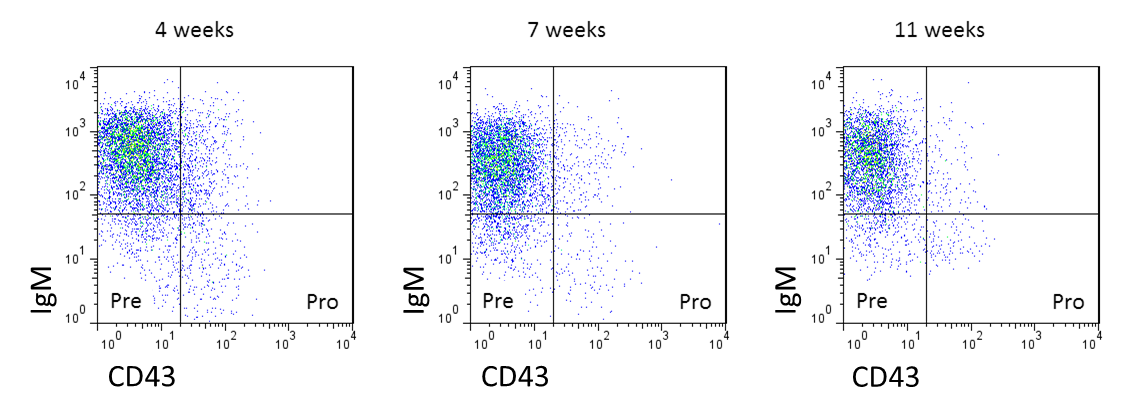
\includegraphics[width=\textwidth]{Figures/NODpropre.png}
	\caption{Pro (IgM\textsuperscript{-}CD43\textsuperscript{+}) and pre (IgM\textsuperscript{-}CD43\textsuperscript{-})B cells are present in thymi of NOD mice at all ages. Plots are representative of several repeats of flow cytometry of NOD mice at the stated ages. Samples are acquired using a CD19 gate which acquires 100\% of all CD19+ cells and ~2\% of CD19- cells. Gating pattern: Lymphocytes, single cells, CD19\textsuperscript{+} then IgM vs CD43 as shown.}
	\label{fig:propre}
\end{figure}

\subsection{Developing B cells in the thymus express RAG}


To try and identify whether or not pro and pre B cells are developing within the thymus rather than migrating there, the expression of RAG in these developing B cells was investigated.
The necessity of RAG expression for BcR rearrangement and subsequent progression to the pre B cell stage means that active RAG expression indicates active development.
To do this, NOD-RAG-GFP reporter mice were used.
These mice express GFP under the RAG promoter so that when RAG transcription is activated, so is GFP.

To identify active RAG expression, the intensity of GFP must be considered.
GFP is a protein with a half-life of ~54 hours therefore the signal will be brightest when it is newly produced.
Lower intensities of GFP suggest recently deactived GFP transcription so that some of the protein will have decayed and thus the signal will have decreased.
For example, a B cell that developed in the bone marrow and moved to the thymus would have expressed GFP in the bone marrow when rearranging their receptor and the GFP intensity would be very bright.
If the B cell then migrated to the thymus, the GFP would have degraded either totally or partly so that the intensity would be much lower.
This means that the GFP signal is a method of determining the likelihood of active development of B cells in the thymus.
An actively developing B cell in the thymus therefore should be GFP\textsuperscript{high}CD19\textsuperscript{+}.

Thymi and bone marrow from NOD-RAG-GFP mice of 4, 7 and 11 weeks of age were used for flow cytometry to look for the presence of RAG\textsuperscript{+}CD19\textsuperscript{+} cells.
Setting the gates for RAG\textsuperscript{high} and RAG\textsuperscript{low} populations was done by looking at the RAG levels in the total thymic tissue including B and T cells.

As shown in \cref{subfig:RAGhighlownegthyB}, it appears that there are CD19\textsuperscript{+}RAG\textsuperscript{+} cells in the NOD thymus at 4, 7 and 11 weeks of age.
As shown in \cref{subfig:RAGhighlowneggraph}, the difference between the CD19\textsuperscript{+}RAG\textsuperscript{high} cells between 4 and 11 weeks is not significant, however the change in CD19\textsuperscript{+}RAG\textsuperscript{low} cells is significant.
This gives the impression that B cell development is decreasing as mice age.
The decreased population of RAGCD19\textsuperscript{low} cells suggests there are less newly developed B cells in the thymus of NOD mice as they get older.
Data was obtained from 4/5 mice of each age group.


\begin{figure}
	\begin{subfigure}{\textwidth}
	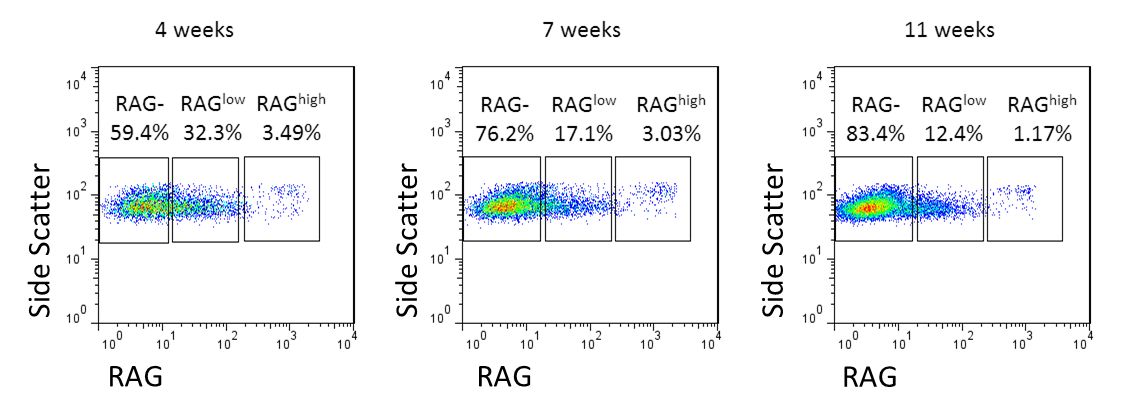
\includegraphics[width=\textwidth]{Figures/RAGhighlownegthyB.png}
	\caption{Thymic B cells expressing RAG}
	\label{subfig:RAGhighlownegthyB}
	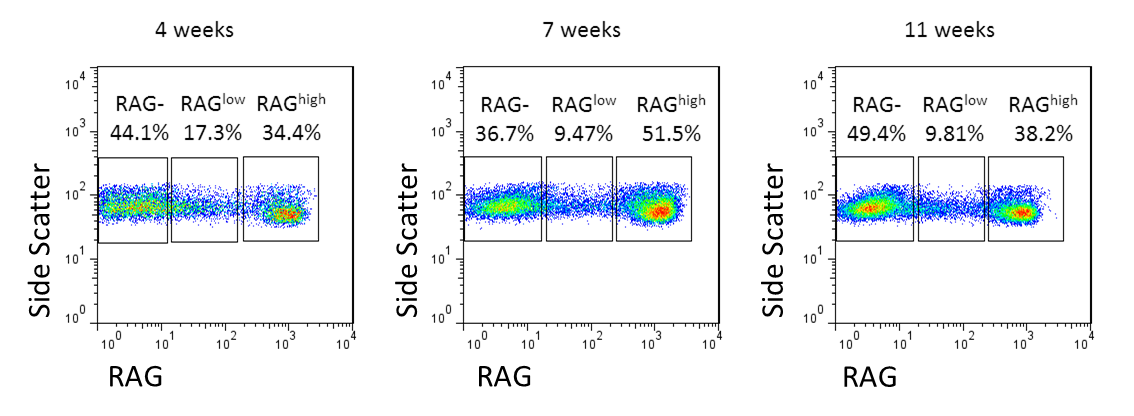
\includegraphics[width=\textwidth]{Figures/RAGhighlownegtotalthy.png}
	\caption{RAG expression in total thymus}
	\end{subfigure}
	\begin{subfigure}{\textwidth}
	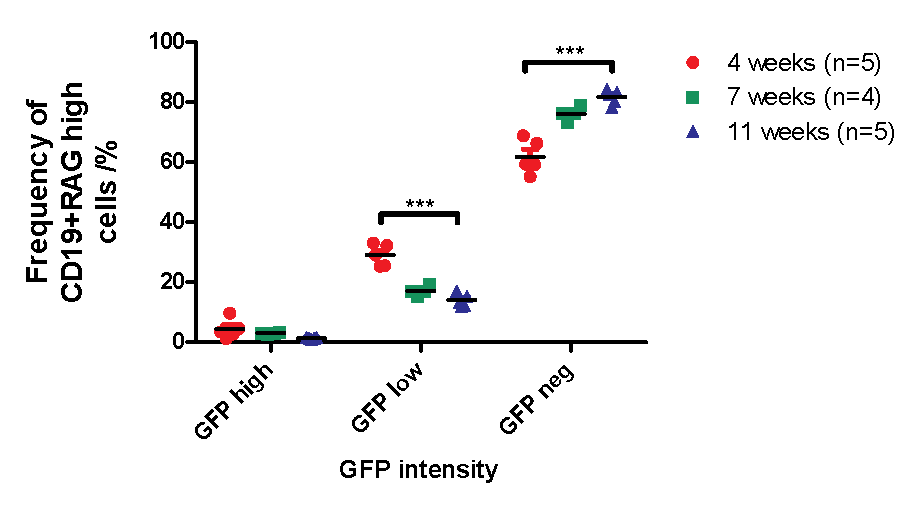
\includegraphics[width=\textwidth]{Figures/RAGhighlownegative.pdf}
	\caption{Frequency of CD19\textsuperscript{+}GFP\textsuperscript{high}, CD19\textsuperscript{+}GFP\textsuperscript{low} and CD19\textsuperscript{+}GFP\textsuperscript{-}. Data analysed with a 1 way ANOVA and Tukey's test for comparison of multiple groups.}
	\label{subfig:RAGhighlowneggraph}
	\end{subfigure}
\caption{CD19+ cells in the NOD thymus express RAG. 
Top panel shows the RAG expression of CD19+ cells in the thymus of NOD-RAG-GFP reporter mice at 4, 7 and 11 weeks of age. Bottom panel shows the total thymic RAG expression used to set gates of RAG\textsuperscript{high}, RAG\textsuperscript{low} and RAG-. 
Gates were then put onto CD19+ population. 
CD19\textsuperscript{+}RAG\textsuperscript{high} cells are likely to be developing B cells as they express CD19 and RAG, suggesting active rearrangement. 
Each age group plot is representative of 4/5 mice of given age.
Gating pattern: lymphocytes, single cells, CD19\textsuperscript{+} (CD19 gate omitted when looking at total thymus RAG expression).}
\end{figure}

\todo{Correct axis labels}


\subsection{B cell development is dependent on the presence of a mature B cell}

Following on from this finding, B cell KO NOD mice thymi were also investigated.
In these mice, as stated in \cref{methods:mice}, these mice are unable to rearrange their IgM heavy chain and therefore cannot progress beyond the pro B cell stage. 
In the bone marrow of these mice, a population of pro B cells is seen, but there are no pre B cells and no IgM\textsuperscript{+} cells.
It was therefore expected that in their thymus there would also be a population of pro B cells, similar to that seen in the NOD WT mice. 
However, this does not appear to be the case.

To investigate the presence of pro B cell frequency between the different mice strains, it was first necessary to determine an appropriate gating system so the strains could be compared fairly.
To final strategy was lymphocytes, single cells, IgM\textsuperscript{-}, CD43\textsuperscript{+} then the frequency of CD19\textsuperscript{+} cells within this population was obtained as the frequency of pro B cells relative to the frequency of IgM\textsuperscript{-}CD43\textsuperscript{+} cells in each strain.

As shown in \cref{subfig:MatureBincproBgraph}, the frequency of pro B cells is significantly decreased in the NOD KO thymi compared to both NOD WT and B6 thymi (Data analysed using a One-Way ANOVA and Tukey's test).
This is an interesting finding as it suggests that the enhancement of pro B cells in the thymus may be dependent on the presence of a mature B cell.
The difference between the NOD WT and B6, however, is not significant suggesting that an increase in pro B cells cannot account for the increase in thymic B cells seen in the NOD WT thymus.

The investigation was carried out in a blind trial so that the strains of mice were not known during analysis in order to avoid bias in the results.

\begin{figure}
	\begin{subfigure}{\textwidth}
	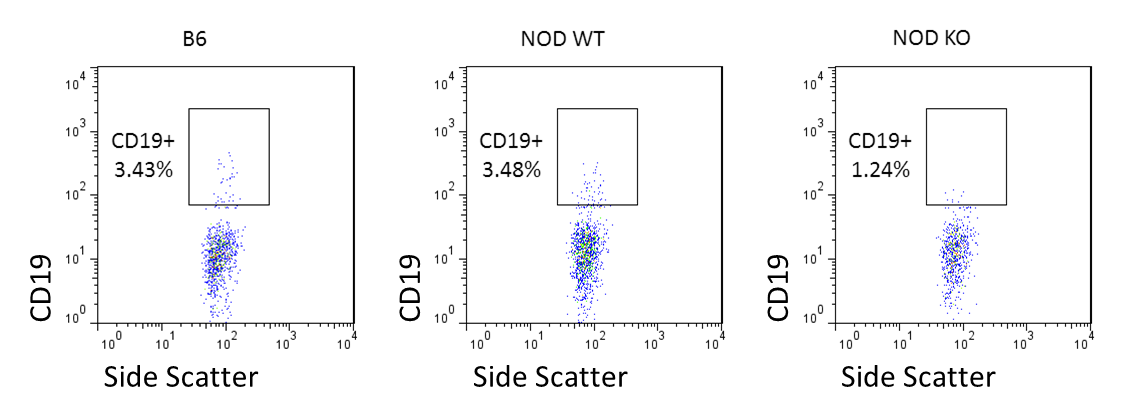
\includegraphics[width=\textwidth]{Figures/MatureBincproB.png}
	\caption{CD19+CD43+IgM- pro B cells in, from left to right, B6 mouse, NOD WT and NOD KO mice of 6-8 weeks of age}
	\end{subfigure}
	\begin{subfigure}{\textwidth}
	\centering
	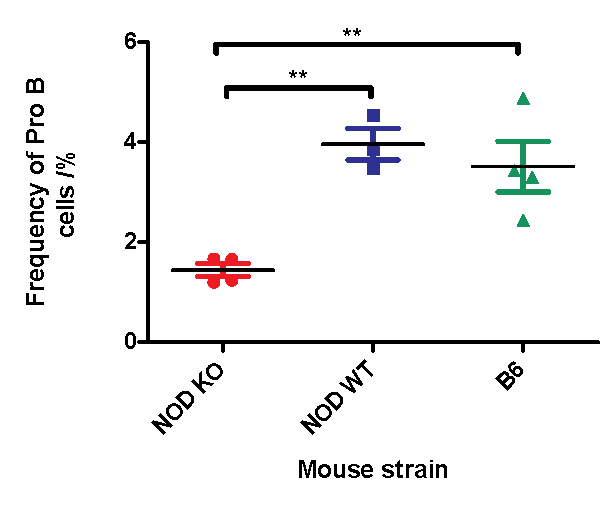
\includegraphics[width=0.6\textwidth]{Figures/MatureBincproBgraph.pdf}
	\caption{Graph to show difference in pro B cell frequency in NOD WT, NOD KO and B6 mouse thymi}
	\label{subfig:MatureBincproBgraph}
	\end{subfigure}
\caption{Mature B cells increase frequency of pro B cells in the thymus.
Top panel shows representative FACS plots showing a decreased frequency of CD19\textsuperscript{+}IgM\textsuperscript{-}CD43\textsuperscript{+} cells (pro B cells) in the thymus.
The bottom panel shows this data in a graph.
Statistical significance was determined using a One-way ANOVA and Tukey's test. NOD KO has a statistically significantly lower frequency of pro B cells compared to both NOD WT and B6 control. NOD WT n=3, NOD KO n=4, B6 n=4. Frequencies shown are percentage of CD19\textsuperscript{+} cells within the IgM\textsuperscript{-}CD43{+} population within the thymus.}
\label{fig:MatureBincProB}
\end{figure}


\subsection{NOD mice express higher levels of CD43 in the thymus}
\label{Results:CD43}

During analysis of data regarding frequencies of pro B cells in the NOD thymus compared to B6 thymi, it was noted that there appeared to be a difference in frequency/intensity of CD43 expression in the different strains.
The frequency of IgM\textsuperscript{-} cells is very similar between B6, NOD WT and NOD KO mice.
However, when the expression of CD43 is investigated within this population, it appears that the expression on NOD mice, both WT and KO, is increased compared to B6 mice, as shown in \cref{fig:CD43expression}.
Statistical analysis shows that only the difference between the KO and B6 is significant.
The graph also shows a wide spread of frequencies for both NOD background strains.
This spread may be decreased by increasing the group size as the number of mice was small.
However, the B6 data is all very close suggesting that the B6 may be a more regimented environment compared to the NOD which could account for the differences in spread of data across the strains.
The experiment was carried out blind so that all strains were analysed without bias.


\begin{figure}
	\begin{subfigure}{\textwidth}
	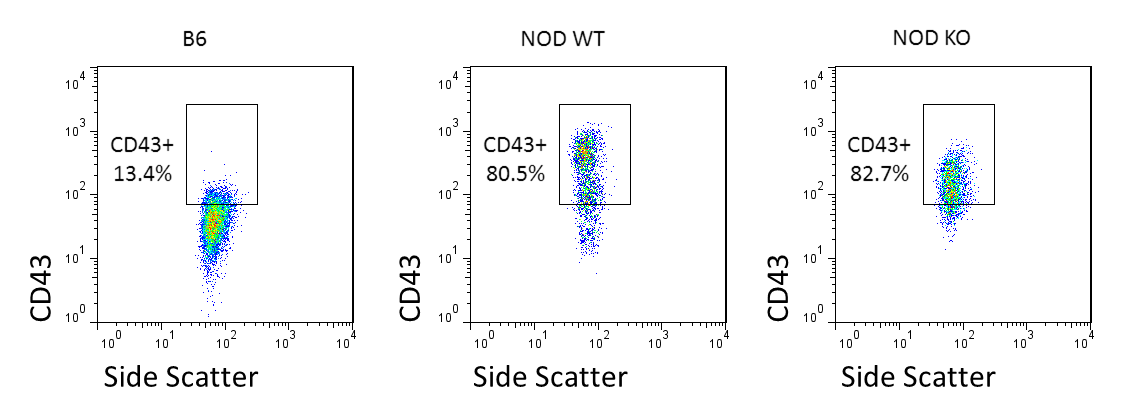
\includegraphics[width=\textwidth]{Figures/CD43expression.png}
	\caption{Figure showing CD43 expression in IgM- cells in the thymus}
	\end{subfigure}
	\begin{subfigure}{\textwidth}
	\centering
	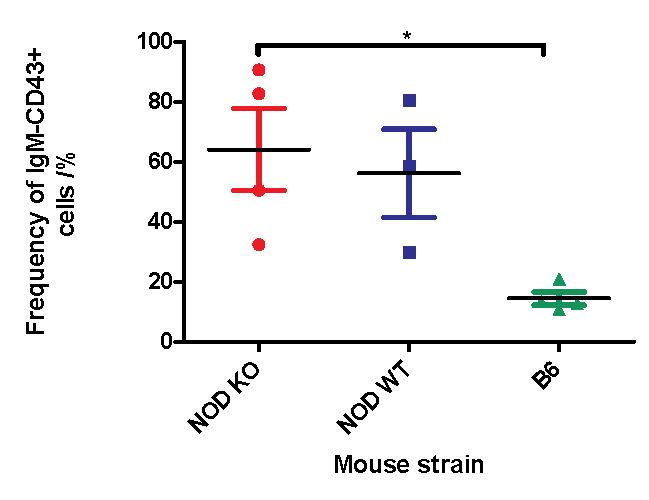
\includegraphics[width=0.6\textwidth]{Figures/CD43levels.pdf}
	\caption{Graph showing increased CD43 expression NOD}
	\end{subfigure}
\caption{NOD mice show increased CD43 expression in the thymus.
Top panel shows representative FACS plots showing increased CD43 expression in NOD WT and NOD KO mice.
However, the graph shows that the difference is only significant between the NOD KO and B6, analysed using a One-Way ANOVA and Tukey's test.
FACS plots gated lymphocytes, single cells, IgM\textsuperscript{-} then analysed on CD43 expression.
NOD KO n=4, NOD WT n=3, B6 n=4. }
\label{fig:CD43expression}
\end{figure}

%CD43 levels on B cells from last year???

\subsection{Transfer}

Following on from the findings that pro B cell frequency is lowered in NOD KO mice, a pilot study was set up whereby thymic cells were injected intravenously into NOD KO mice.
The thymi from two donor NOD WT mice were taken and split into CD19+ and CD19- fraction using MACS.
This was to see if the presence of thymic cells, with or without CD19+ cells, had any effect on the presence of pro B cells in the KO thymus.

Due to the preliminary nature of this transfer experiment, very small numbers of mice were used.
2 donor mice were taken and split into CD19+ and CD19- fractions and the fractions were then pooled.
4 recipient mice were used, 2 received CD19+ fraction cells and 2 received CD19- fraction cells.
One recipient each for each fraction were taken at 7 days for analysis and the others were taken at 11 days post transfer.
Tissues taken for analysis were bone marrow, thymus, spleen, pancreas, pancreatic lymph node and lateral axillary lymph node.
The numbers/phenotypes of donor cells are shown in \cref{subfig:WTdonortable}.

\todo{Diagram explaining set-up of experiment}


The experiment was of interest due to the fact a similar thing has been attempted before by \citet{Serreze1998}, whereby NOD B cells were injected into NOD KO recipient mice.
Interestingly, it was found that the transferred B cells disappeared in the recipient mice between 6-11 days post transfer, hence the 7 and 11 day timepoints for analysis.
However, the difference was that the injected B cells were conventional splenic B cells.
Here in my transfer experiment, the transferred cells were of thymic origin and since relatively little is known about thymic B cells, it was wondered whether the outcome would be the same. 
Therefore, the aim of the experiment was 2 fold, one, to see if thymic B cells could survive transfer and two, to see if the presence of thymic B cells had an effect on the frequency of pro B cells in the KO thymus.

Interestingly, in concordance with \citet{Serreze1998}, analysis revealed that mature B cells were only present in the recipient mice at the 7 day post transfer time point, see \cref{fig:Transfer}.
Bone marrow, thymus, spleen, pancreas, pancreatic lymph node and axillary lymph nodes were all analysed to look for donor B cell presence, however, B cells are only seen in the the thymus and spleen at the 7 day time point.
No B cells were seen in any of the tissues at the 11 day time point.
This is similar to the findings of \citet{Serreze1998} and could suggest that the B cells are being killed off by cytotoxic T cells which have never developed tolerance to B cells due to their absence during T cell development.
On the other hand, due to the fact that the group size is very small, one mouse per group, the results must be viewed with caution.

Although B cells are seen in the thymus and spleen of both recipients at the 7 day time point, it seems that there is a higher frequency of CD19\textsuperscript{+}IgM\textsuperscript{+} cells in the CD19\textsuperscript{+} recipient.
This finding is not surprising as this recipient received mature B cells in the transferred cells.
However, there are still some B cells seen in the CD19\textsuperscript{-} recipient.
These could be B cells that developed from CD19\textsuperscript{-} progenitors which were injected or they may be contaminating B cells that were transferred.

\begin{figure}
	\begin{subfigure}{\textwidth}
	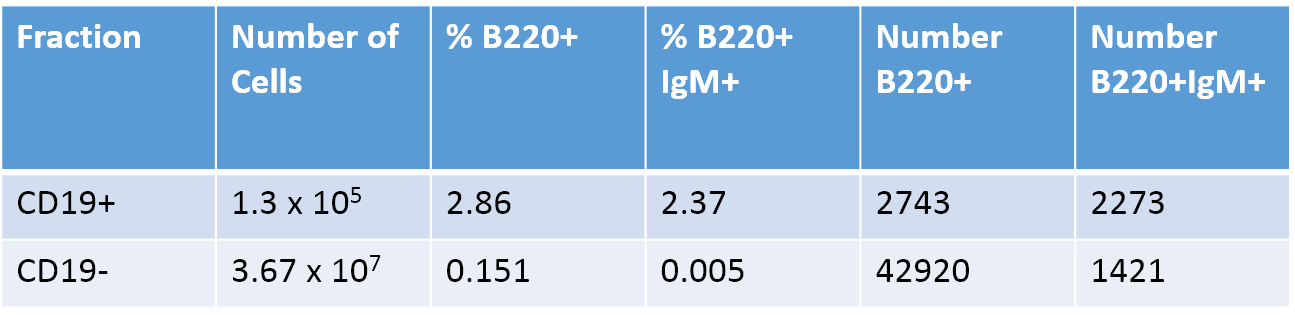
\includegraphics[width=\textwidth]{Figures/WTdonortable.png}
	\caption{Donor cell numbers and phenotypes}
	\label{subfig:WTdonortable}
	\end{subfigure}
	\begin{subfigure}{\textwidth}
	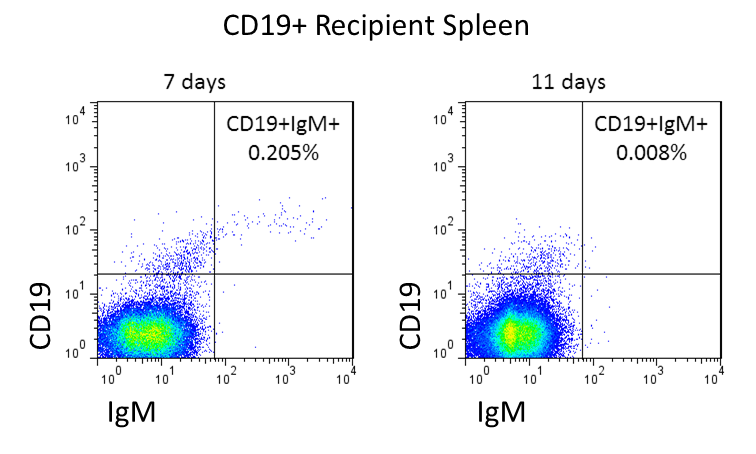
\includegraphics[width=0.5\textwidth]{Figures/CD19posrecipspleen.png}
	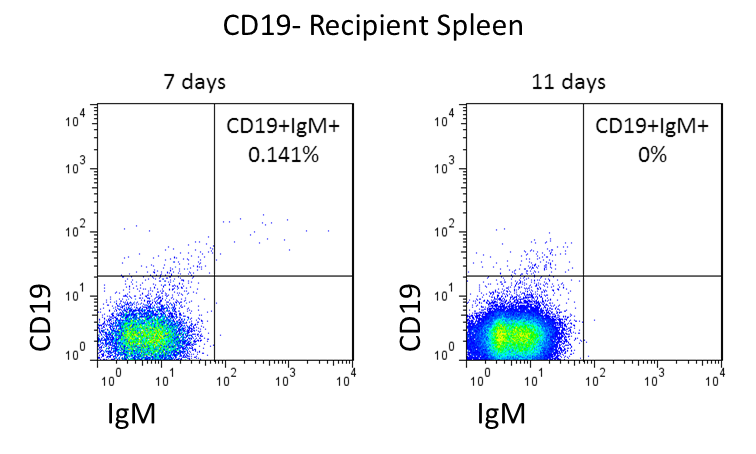
\includegraphics[width=0.5\textwidth]{Figures/CD19negrecipspleen.png}
	\caption{Spleen of recipient mice showing frequency of CD19+IgM+ B cells at 7 and 11 days post transfer}
	\end{subfigure}
	\begin{subfigure}{\textwidth}
	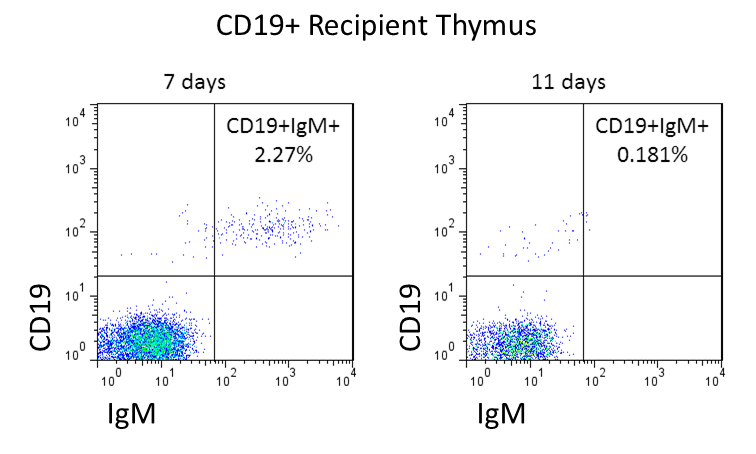
\includegraphics[width=0.5\textwidth]{Figures/CD19posrecipthy.png}
	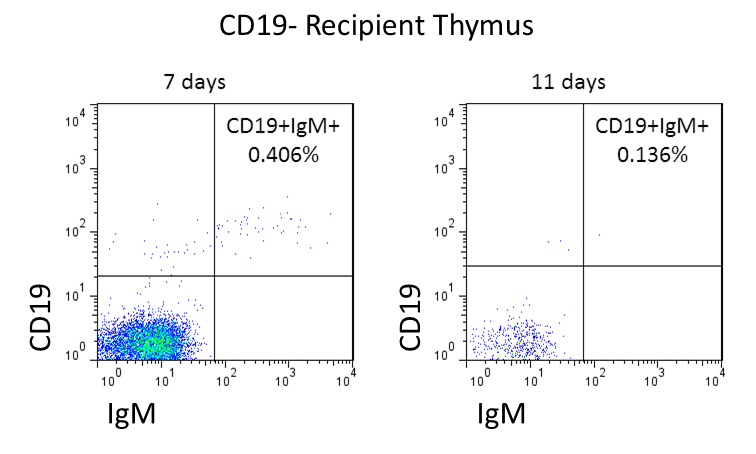
\includegraphics[width=0.5\textwidth]{Figures/CD19negrecipthy.png}
	\caption{Thymus of recipients showing B cell presence/absence at 7 and 11 days post transfer}
	\end{subfigure}
\caption{Figure showing B cell presence/absence in spleen and thymus over time.
Top panel shows B cell presence in the spleen of the CD19+ and CD19- recipients at 7 and 11 days post transfer.
Bottom panel shows the same but in the recipient thymi.
Data shown is gated lymphocytes, single cells, GFP\textsuperscript{+} then analysed on CD19 expression.
n=1 for every group.}
\label{fig:Transfer}
\end{figure}

\subsubsection{Is there an effect on the number of pro B cells?}

It was then wondered whether or not the recipient KO mice had an increase in pro B cells in the thymus due to the effect of transferred B cells.
However, it appears that there is no difference in the frequency of pro B cells between the KO control and either recipient (Data not shown).
The results were also very varied and inconsistent therefore the group sizes would need to be increased significantly and the experiment repeated in order to obtain any meaningful results.

Whilst the experiment was inconclusive, it was a good starting point in that the transfer itself worked well, all the recipients survived transfer and evidence of the transferred cells could be seen in the recipients at least 7 days post transplant.
This method therefore may be a good way for invesigating thymic B cell migration following intravenous transfer.
In order to improve validity of results, it would be important to increase the group sizes and it may be beneficial to move the time points forward as this could give a better picture of thymic B cell migration before they disappear.

However, the results suggest that is may not be the way to study the effect of mature B cells on the enhancement of the pro B cell population.
As suggested by \citet{Serreze1998}, it may be neccesary to irradiate mice and then transplant bone marrow supplemented with mature B cells so that the T cells that come from the transplanted bone marrow will develop and be tolerised to the B cells.

Following these improvements, if there still is truly no difference in pro B cell frequencies between NOD KO controls and KO with B cells, it may suggest one of many possibilities as follows:
\begin{itemize}
\item The mature B cell(s) required to increase the pro B cell frequency must be endogenous to the host
\item The mature B cell(s) must not be of thymic origin
\item During transfer, the property required by a mature B cell to increase pro B cell frequency, is lost
\item Transfer may not provide enough B cells to influence pro B cell presence in the thymus
\item B cells may have been killed off in the recipient before they had a chance to influence the thymic pro B cell compartment
\end{itemize}

Clearly, more extensive research into this area is required to increase our understanding of the effects of a mature B cell on developing B cells in the thymus.


\subsection{Early B cell progenitors are present in the NOD thymus}

\subsubsection{Introduction to progenitor work}

Given the significant increase in thymic B cells in the NOD mouse compared to controls, it was decided that investigation into the presence of early B cell progenitors would be beneficial.
In particular, whether or not there is a difference in frequencies of early B cell progenitors, similar to the picture seen in pro B cells.

For this, it was important to first of all decide on the specific progenitor that would be looked for.
Although the B cell commitment pathway remains undefined, as mentioned in \cref{subsec:Bcelldevelopment}, it appears that a so-called BLP may be the best described B cell progenitor.
In which case, the cells of interest would be Sca-1\textsuperscript{low} c-kit\textsuperscript{low} Flt3\textsuperscript{+} IL-7Ra\textsuperscript{+} Ly6D\textsuperscript{+} \citep{Mansson2010, Inlay2009, Zhang2013}.

However, the matter was complicated further due to the fact research into B cell commitment and development is focussed normally on normal development within the bone marrow.
Research into the development of B cells in the thymus, therefore, requires the assumption that the developmental pattern will match that of the bone marrow.
While it is not known how well the developmental pattern in the thymus mirrors that of the bone marrow, it is a good place to start due to the wealth of literature relating the B cell development in the bone marrow.

The aim of the experiment was to determine whether or not the frequencies of BLPs in the NOD mouse were the same as that seen in the non diabetic B6 control and in the NOD KO.
This would give insight into two areas.
Firstly, do NOD mice have an increased frequency of B cell progenitors in their thymus compared to B6 mice which could potentially explain the increased number of B cells in the NOD thymus.
And secondly, are BLPs affected in the same way as pro B cells by the presence or absence of a mature B cell shown by a decreased frequency of BLPs in the NOD KO compared to the NOD.

%To investigate this, flow cytometry was used which included a wide range of antibodies to assess BLP presence.
%The antibodies used are as follows:
%\begin{itemize}
%\item CD4/CD8 - These were used to gate out any residual mature T cells that had not been removed through MACS depletion
%\item Sca-1 - Downregulates from high on HSCs to low on CLPs
%\item c-kit - Downregulates from high on HSCs to low on CLPs
%\item Flt3 - Upregulates from negative on HSCs to high on CLPs then becomes negative again on B cells \citep{Holmes2006}
%\item IL-7Ra - Upregulates on LMPPs to being high on CLPs.
%\item Ly6D - Correlates with B cell lineage restriction \citep{Inlay2009}
%\end{itemize}

%Theoretically, this stain should allow analysis of all progenitor populations from HSCs through MPPs, LMPPs, CLPs, ALPs to BLPs.

Mice used were 6-8 weeks old.
This age was chosen as this is the point that B cells start to significantly increase compared to B6 controls.
Therefore, it is a good point to investigate the development of the B cells as any differences between the two strains should be most apparent.



\subsection{Magnetic-assisted cell sorting optimisation}

Due to the small size of progenitor populations in comparison to mature cell populations in the thymus, it was first necessary to deplete the thymus of the majority of mature cells before looking for progenitors.
For depletion, magnetic-activated cell sorting (MACS) was used.
There are many different kits available and the decision on which to use for the experiments was taken after investigating the efficiency and yield from Miltenyi beads and columnms, and Qiagen anti-rat beads \todo{name of Qiagen beads}

Firstly, Miltenyi columns and lineage depletion beads were tested to assess their efficiency.
To start with, only one round of depletion was carried out which gave an efficiency of \todo{look at efficiencies}, see \cref{subfig:1rounddep}.
This efficiency was improved to \todo{add efficiency of 2 rounds} when two rounds of depletion were carried out \cref{subfig:2rounddep}. 
However, while this method gave a very pure sample with very few mature cells remaining, the yield was not very good.

\begin{figure}
	\begin{subfigure}{\textwidth}
	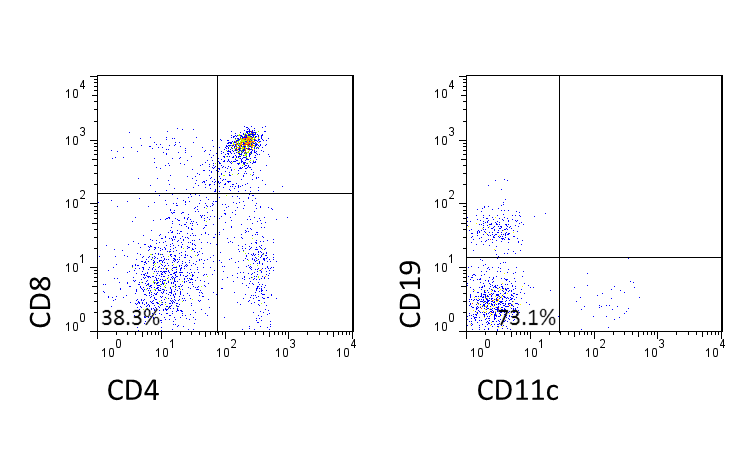
\includegraphics[width=0.8\textwidth]{Figures/1rounddepletion.png}
	\caption{One round of depletion using Miltenyi lineage depletion beads and columns}
	\label{subfig:1rounddep}
	\end{subfigure}
	\hfill
	\begin{subfigure}{0.8\textwidth}
	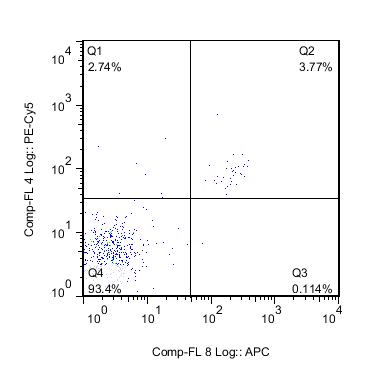
\includegraphics[width=\textwidth]{Figures/2rounddepletion.png}
	\caption{Two rounds of depletion using Miltenyi lineage depletion beads and columns}
	\label{subfig:2rounddep}
	\end{subfigure}
	\hfill
	\begin{subfigure}{0.8\textwidth}
	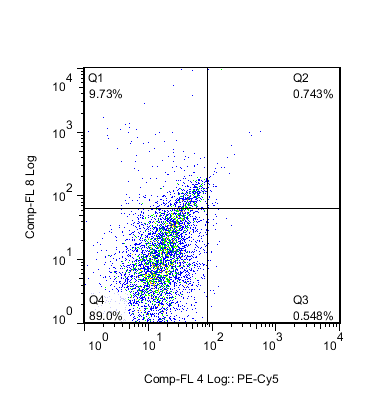
\includegraphics[width=\textwidth] {Figures/Qiagenbeads.png}
	\caption{Qiagen Beads}
	\label{subfig:Qiagen}
	\end{subfigure}
	
\caption{Figure showing the different methods of depletion. 
Methods for each outlined in \cref{Methods:MACSdepletion}.
FACS plots gated lymphocytes, single cell CD4\textsuperscript{-}CD8\textsuperscript{-}, then for Miltenyi methods CD19\textsuperscript{-}CD11c\textsuperscript{-} and for Qiagen beads B220\textsuperscript{-}.}
\end{figure}

Qiagen beads were also tested as an alternative to the Miltenyi kits. 
As shown in \cref{subfig:Qiagen}, the efficiency of this method was also very good and the yield was also much improved compared to the Miltenyi beads therefore this was the chosen method of depletion.


\subsection{BLPs are present in NOD mouse}

The gating pattern used for the experiment is shown in \cref{subfig:BLPgating}.
Firstly Lymphocytes and single cells were identified (Not shown) and then CD4\textsuperscript{-}CD8\textsuperscript{-} cells were taken forward to be analysed as shown.

Interestingly, the analysis gave very inconsistent results for both the WT and KO NOD mice, as shown in \cref{subfig:BLPgraph}.
The frequencies of each population of cells varied widely over the 3 NOD WT and 4 NOD KO. 
For example, while the frequencies of Sca-1\textsuperscript{low} and c-kit\textsuperscript{low} remained fairly similar for both KO and WT, beyond this point, the percentages of IL-7Ra\textsuperscript{+}, Flt3\textsuperscript{+} and Ly6D\textsuperscript{+} showed a large amount of variation.
However, the same was not seen in the B6 control mice.
These mice showed very consisten frequencies of each population.

Whilst the data is not hugely useful in determining difference in presence of B cell progenitors, it does suggest that in the B6 mouse, the pattern of development is very well controlled and therefore consistent between mice.
This contrasts with the mice of NOD background which show huge variablity suggesting that the pattern of development in these mice is much less well controlled.
This potential lack of control could be contributing to the increase in B cells in the thymus.

However, despite the variable data from the NOD mice, the data may suggest that actually there are more BLPs present in the B6 mouse compared to the NOD mouse.
This is surprising due to the far increased population of B cells seen in the NOD thymus.
This could suggest that B cells are actually developing in a different way in the thymus compared to the bone marrow in the NOD mouse, and potentially a different way to the normal physiological B cells seen in the B6 thymus.
With this is mind, other potential B cell development patterns must be explored.

\begin{figure}
	\begin{subfigure}{\textwidth}
	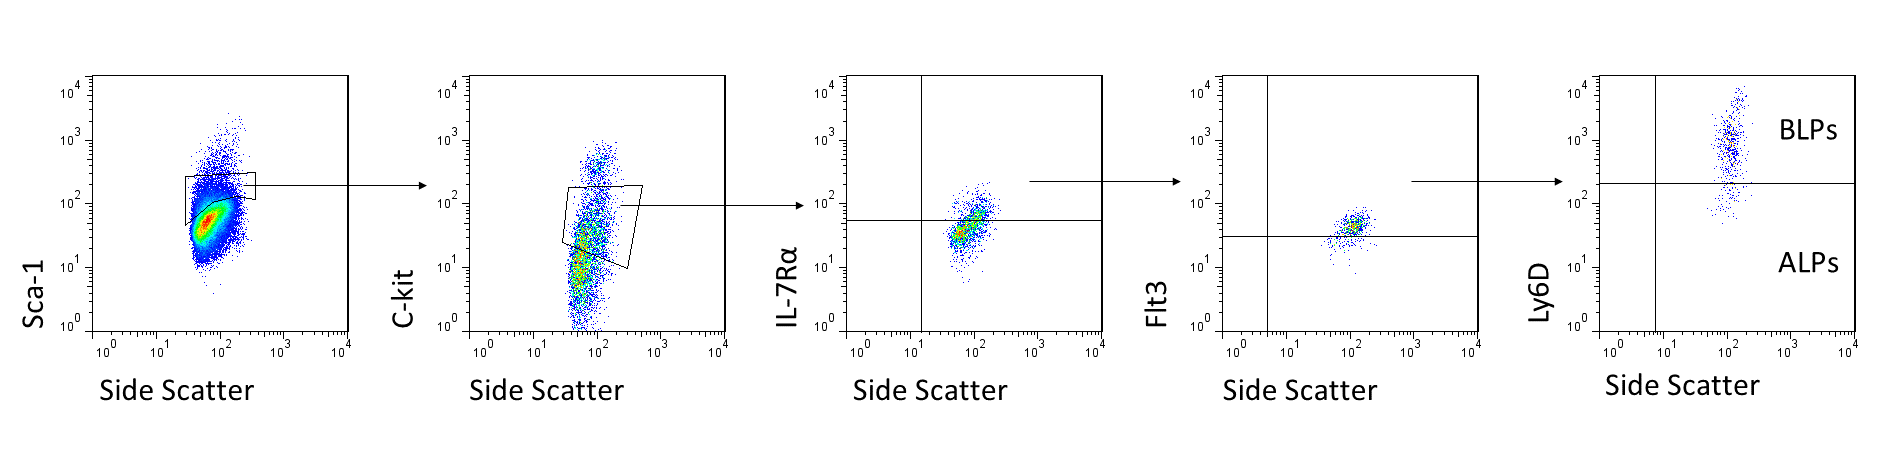
\includegraphics[width=\textwidth]{Figures/BLPgating.png}
	\caption{Gating pattern used to identify BLPs}
	\label{subfig:BLPgating}
	\end{subfigure}
	\begin{subfigure}{\textwidth}
	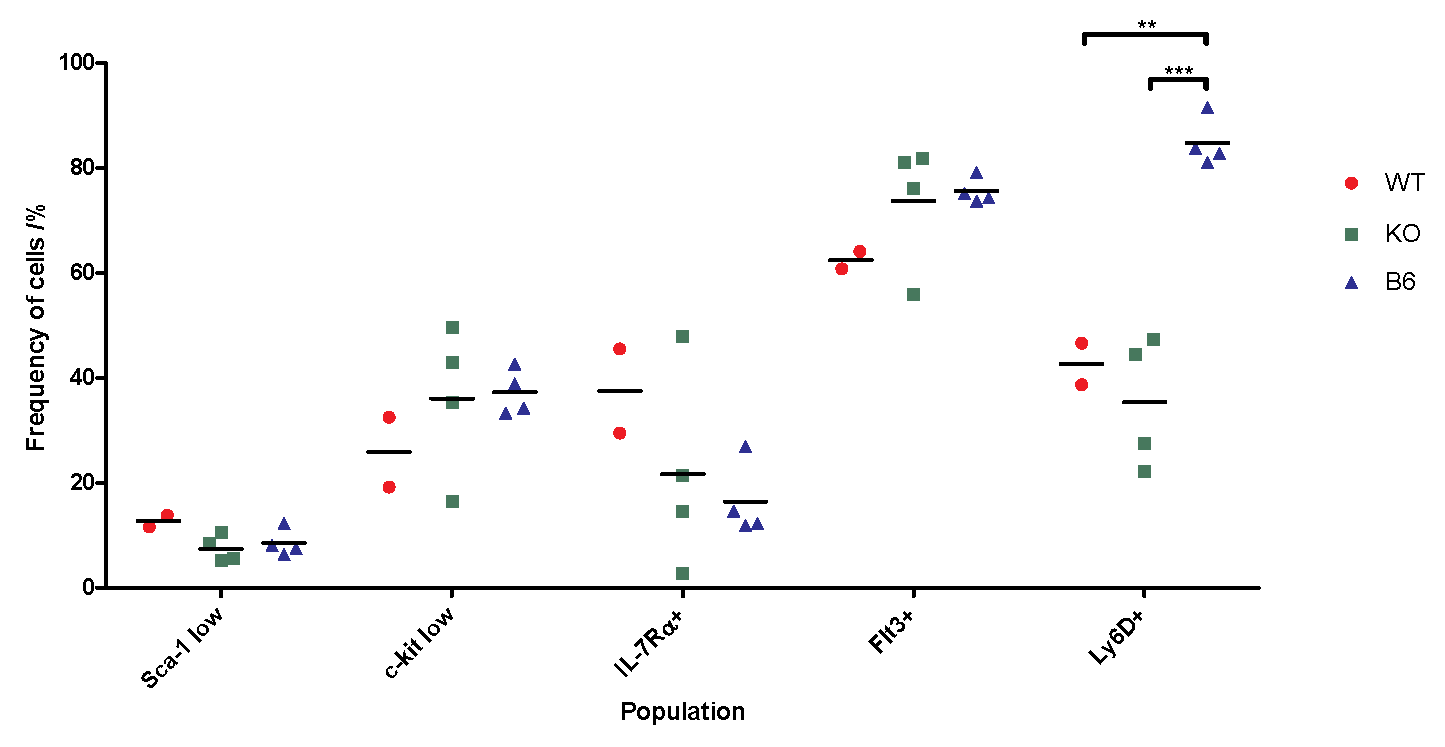
\includegraphics[width=\textwidth]{Figures/ProgenitorMarkers.pdf}
	\caption{Graph showing the frequencies of cells expressing each marker at the appropriate level.}
	\label{subfig:BLPgraph}
	\end{subfigure}
\caption{BLPs are present in the NOD thymus. 
Top panel shows gating pattern to look for BLPs in the thymus of mice. Lymphocyte and single cell gate not shown.
Bottom panel shows the frequency of each marker within the population of the previous marker.
One way ANOVA and Tukey's test carried out on Ly6D\textsuperscript{+} population revealing a significantly increased population of BLPs in the B6 mice compared to both NOD WT and NOD KO.
11 mice were used, all aged 6-8 weeks. 
The experiment was carried out blind to avoid bias. 
NOD WT n=3, NOD KO n=3, B6 n= 4.}
\label{fig:BLPs}
\end{figure}

\todo{Swap IL-7R$\alpha$ and Flt3 round on graph}





%\subsection{T cell development looks normal/abnormal in NOD mouse compared to control}
%\fig{CD4 v CD8 in NOD, KO and B6 (and FVB). Different ages, 5,9,12wks?}
%\fig{Graphs of DP, DN and SP}

%\todo{analyse data to see whether it is normal or abnormal. This is a good control to give an indication of the overall condition of the thymus, preferably over time to see how it changes as mouse ages with normal physiological atrophy of the thymus}

\subsection{The NOD thymus contains B cell development transcription factors}

If B cells are developing within the thymus, this begs the question as to whether the NOD thymus is providing an environment more conducive to B cell development compared to nondiabetic controls. 
To investigate this, primers were designed that were specific for B cell development factors such as E2A, EBF, Pax5, VPreB and CXCL12.
%\todo{look in Hagman2006, Welinder2011, Mansson2008, Cobaleda2007, Radtke2013, Riley2013, Tokoyoda2004 for TF info}.

To date, only non-quantitative PCR has been carried out to compare whether or not B cell development transcription factors are present in the NOD bone marrow and thymus.
Since normal B cell development occurs in the bone marrow, these transcription factors would be expected there and indeed they were seen there, as shown in \cref{fig:gels}. 
Interestingly, all the genes, besides CXCL12, were also present in the NOD thymus too.
This indicates that the thymic environment may also be allowing B cell development.
The lack of CXCL12 in the thymus is not a surprising result as it is a cytokine responsible for holding developing B cells in the bone marrow niche and therefore, may be more bone marrow specific rather than B cell specific.

\begin{figure}
	\begin{subfigure}{0.5\textwidth}
	\centering
	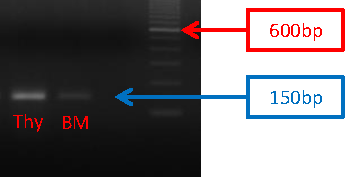
\includegraphics[width=\textwidth]{Figures/E2A.pdf}
	\caption{E2A}
	\end{subfigure}
	\begin{subfigure}{0.5\textwidth}
	\centering
	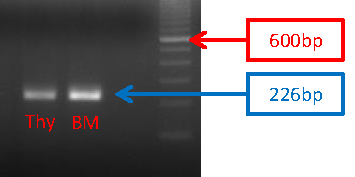
\includegraphics[width=\textwidth]{Figures/EBF.pdf}
	\caption{EBF}
	\end{subfigure}
	\begin{subfigure}{0.5\textwidth}
	\centering
	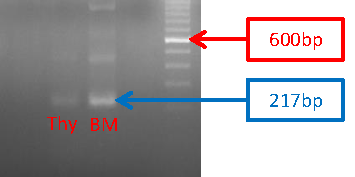
\includegraphics[width=\textwidth]{Figures/sPax5.pdf}
	\caption{Pax5}
	\end{subfigure}
	\begin{subfigure}{0.5\textwidth}
	\centering
	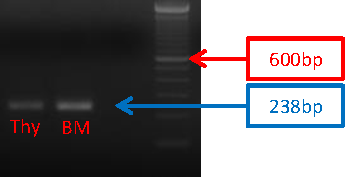
\includegraphics[width=\textwidth]{Figures/VPreB.pdf}
	\caption{VPreB}
	\end{subfigure}
	\begin{subfigure}{\textwidth}
	\centering
	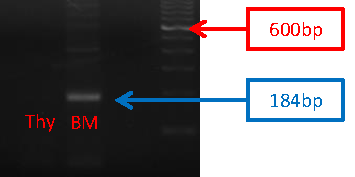
\includegraphics[width=0.5\textwidth]{Figures/CXCL12.pdf}
	\caption{CXCL12}
	\end{subfigure}
\caption{B cell development transcription factors are present in NOD thymi.
Gel electrophoresis of non-quantitative PCR products shows presence of B cell development transcription factors.
Lanes from left to right; Thymus, Bone marrow, 100 bp marker. 
600bp mark showed in red box.
Expected product size is shown in blue box.
Gels were run in 3\% agarose in 1 x TAE buffer. Gels supplemented with 1 $\mu$L ethidium bromide per 25 $\mu$L of 1 x TAE buffer. Gels run at constant 70V. }
\label{fig:gels}
\end{figure}



\subsection{Conclusion}

Data to date has so far given evidence that B cells are developing intrathymically in the NOD mouse.
This is shown by pro and pre B cells being present suggesting that developing B cells are present in the thymus.
Further to this, some of these cells show evidence of active RAG expression, indicating that they are actively developing within the thymus rather than having migrated there following premature release from the bone marrow.

There is also evidence to suggest that B lineage committed early progenitors, such as BLPs, are present within the NOD thymus. 
This also gives the impression that B cells are developing from progenitors within the thymus as these are believed to be the progenitors that pro B cells are derived from.
However, the fact that there are less BLPs in the NOD thymus compared to the B6 could suggest that B cells in the thymus are not developing in the same way as B cells developing in the bone marrow.

Finally, it appears that the NOD thymus may be providing factors that are allowing, if not driving, B cell development.
However, it remains to be seen whether this is a normal finding in nondiabetic controls also.
It would also be useful to carry out quantitative PCR of B cell development factors to see the relative levels between the thymus and bone marrow and across strains of mice.
This could suggest whether or not it may be a thymic abnormality in the NOD mouse which is providing a particularly good environment for B cell development compared to other strains of mice.

\section{Some RAG+ cells in the thymus express B and T cell markers}
During analysis of data from previous experiments, it was noted that a large proportion of RAG+CD19+ cells in the NOD thymus, were also CD4+CD8+.
This was of interest and was therefore investigated further as it indicated there is a possibility for cells with markers of both T and B cells.

\subsection{A large proportion of RAG+CD19+ cells in the NOD thymus express CD4 and CD8}

Having seen RAG\textsuperscript{high}CD19\textsuperscript{+} cells in the NOD thymus suggesting active development of B cells, it was then noted that a large percentage of these cells were also CD4\textsuperscript{+}CD8\textsuperscript{+} \cref{subfig:ThyRAGCD19DP}.
This was an interesting finding as it suggests there may be a point where cells are not yet fully lineage committed and are expressing markers of both T (CD4, CD8) and B (CD19) cells.
These cells all have a high GFP signal and therefore are actively transcribing the protein, indicating that RAG is also active.
This suggests that these cells are expressing markers of both T and B cells as well as rearranging a receptor, though it is not possible to tell which one.

Unfortunately, due to lack of control mice of the correct age, it is not possible to say whether this is a normal pysiological process seen in nondiabetic control mice as well as NOD mice or whether it is unique to the NOD.
Repetitions of the experiments would need to be carried out with the inclusion of B6 control mice.
However, due to normal B cell development occurring in the bone marrow, the thymus and bone marrow were compared for presence of RAG\textsuperscript{+}CD19\textsuperscript{+}CD4\textsuperscript{+}CD8\textsuperscript{+} cells and the bone marrow served as a tissue control.

4 and 7 week old mice were analysed and a representative 4 week old NOD thymus and bone marrow are shown in \cref{fig:RAGCD19DP}. 
Here, the difference between the thymus \cref{subfig:ThyRAGCD19DP} and bone marrow \cref{subfig:BMRAGCD19DP} is shown.
While the thymus contains a significant population of RAG\textsuperscript{high}CD19\textsuperscript{+}CD4\textsuperscript{+}CD8\textsuperscript{+} cells, the bone marrow contains none.

The lack of RAG\textsuperscript{high}CD19\textsuperscript{+}CD4\textsuperscript{+}CD8\textsuperscript{+} cells in the bone marrow suggests it is unlikely that these cells are a normal part of B cell development due to the bone marrow being the normal B cell development site.
It is also unlikely that they are a normal part of T cell development as T cell commitment is thought to occur fully in the DN development stage, therefore when developing T cells are still CD4\textsuperscript{-}CD8\textsuperscript{-}.

This suggests that they are thymus specific and it may highlight another abnormality within the NOD thymus that may or may not be related to the increased population of thymic B cells.
It could potentially suggest an alternative mechanism by which B cells are increased in the NOD thymus, and that is that a cell is beginning to commit to the T cell lineage, then at some point receiving a signal which is causing it to begin to switch lineages and start expressing B cell markers.
This potential redifferentiation could explain the existence of both B and T cell markers on the cells. 
However, further research would be required to explore this further.

These cells are present in NOD mice at both 4 and 7 weeks of age and it was therefore investigated whether or not there was a significant difference in the percentages of these cells between the two age groups. 
The bone marrow is also included in the figure as a comparison.
However, the results show that there is no difference in presence of RAG\textsuperscript{high}CD19\textsuperscript{+}CD4\textsuperscript{+}CD8\textsuperscript{+} cells between the two ages.


\begin{figure}	
	\begin{subfigure}{\textwidth}
	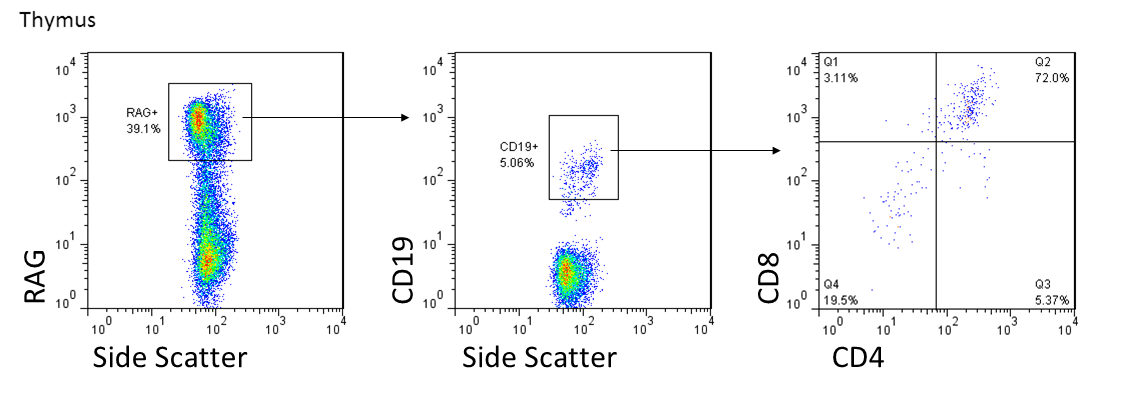
\includegraphics[width=\textwidth]{Figures/Thymus1RAGCD19DP.png}
	\caption{Thymus}
	\label{subfig:ThyRAGCD19DP}
	\end{subfigure}
	\begin{subfigure}{\textwidth}
	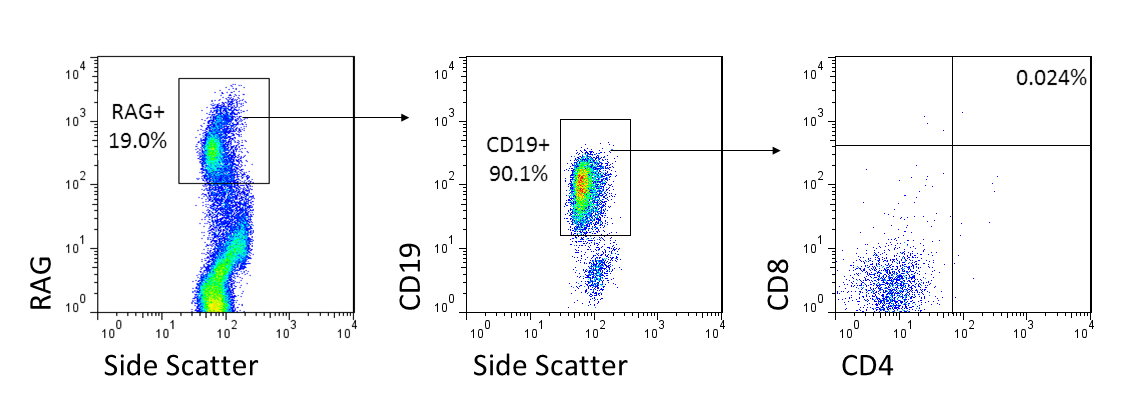
\includegraphics[width=\textwidth]{Figures/BM1RAGCD19DP.png}
	\caption{Bone marrow}
	\label{subfig:BMRAGCD19DP}
	\end{subfigure}
	\begin{subfigure}{\textwidth}
	\centering
	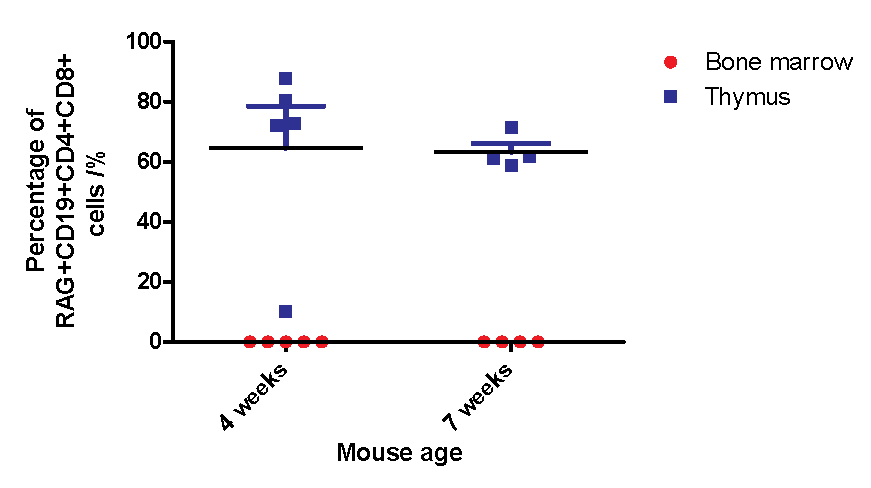
\includegraphics[width=0.8\textwidth]{Figures/BMvThyDP.pdf}
	\caption{}
	\label{BMvThyDPgraph}
	\end{subfigure}
\caption{RAG\textsuperscript{+}CD19\textsuperscript{+}CD4\textsuperscript{+}CD8\textsuperscript{+} cells are present in the NOD thymus but not bone marrow.
Top panel shows representative FACS plot of presence of these cells in the thymus. A CD19 gate was used on acquisition of data so that 100\% of CD19\textsuperscript{+} cells were acquired with only ~2\% of CD19\textsuperscript{-} cells.
Middle panel shows absence of the cells in the bone marrow.
Bottom panel shows no significant difference in frequency of these cells between 4 and 7 weeks of age in the thymus.
Also shows the lack of RAG\textsuperscript{+}CD19\textsuperscript{+}CD4\textsuperscript{+}CD8\textsuperscript{+} cells in the bone marrow.
4 week old NOD-RAG-GFP n=5, 7 week old NOD-RAG-GFP n=4.}
\label{fig:RAGCD19DP}
\end{figure}


\subsection{RAG\textsuperscript{+}IgM\textsuperscript{+}TcR$\beta$\textsuperscript{+} cell presence in the NOD thymus}

Following the finding of RAG\textsuperscript{+}CD19\textsuperscript{+}CD4\textsuperscript{+}CD8\textsuperscript{+} cells in the thymus, it was then of interest to see if these cells with characteristics of both T and B cells progressed to expressing both a TcR and BcR.
This would suggest that these cells were somehow continuing further down the developmental pathway and that the Rag was activated and rearranging both a T and B cell receptor.

To investigate this, the RAG\textsuperscript{+}CD19\textsuperscript{+} were interrogated to see if any expressed both IgM and TcR$\beta$.
As shown in \cref{fig:RAGIgMTcRpos}, it appears that there is a very small population of RAG\textsuperscript{+}IgM\textsuperscript{+}TcR$\beta$\textsuperscript{+} in the thymi of NOD WT mice.
None can be seen in the NOD KO which is unsurprising as they are unable to make IgM.
Data for the bone marrow is not shown as none of the samples showed any RAG\textsuperscript{+}IgM\textsuperscript{+}TcR$\beta$\textsuperscript{+} cells at all (Frequencies = 0\%).

This gives the impression that the RAG\textsuperscript{+}CD19\textsuperscript{+}CD4\textsuperscript{+}CD8\textsuperscript{+} cells do not progress to displaying both a T and B cell receptor.
This could suggest that these cells are just late at committing to a lineage, or it may be that they are the mid point of either a T or B cell transitioning to the other.


\begin{figure}
	\begin{subfigure}{\textwidth}
	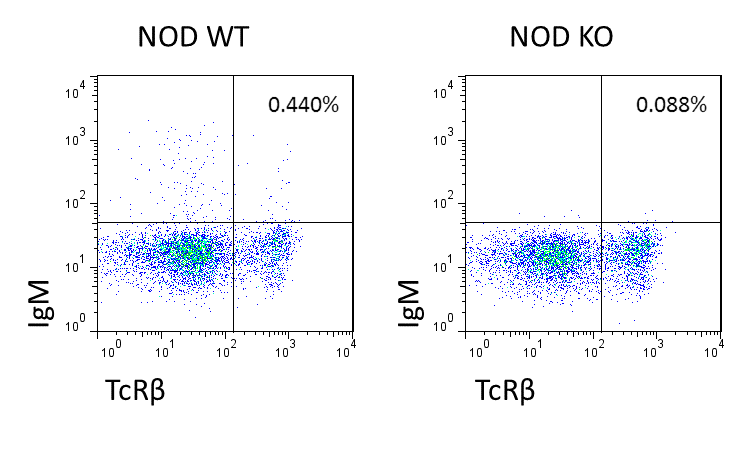
\includegraphics[width=\textwidth]{Figures/ThyRAGIgMTcR.png}
	\caption{Representative NOD WT and NOD KO thymi looking for RAG+IgM+TcR+ cells}
	\label{subfig:BMvThyRAGIgMTcR}
	\end{subfigure}
	\begin{subfigure}{\textwidth}
	\centering
	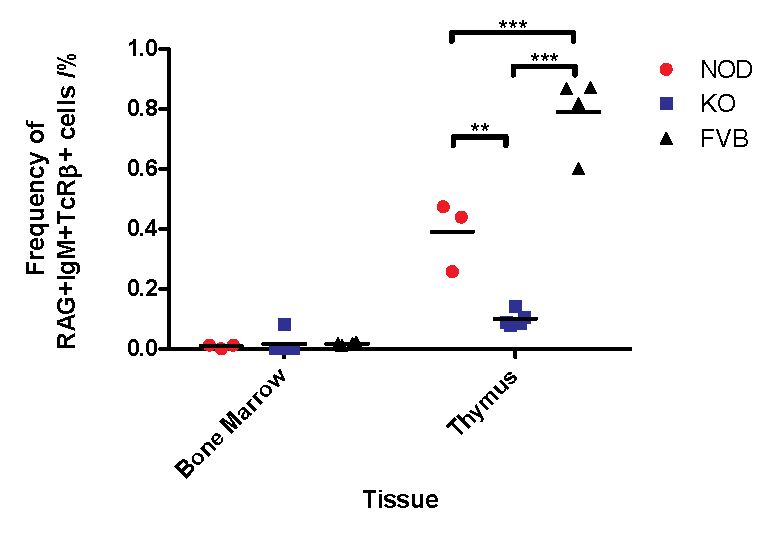
\includegraphics[width=0.8\textwidth]{Figures/IgMTcRposgraph.pdf}
	\caption{}
	\label{subfig:IgMTcRposgraph}
	\end{subfigure}
\caption{There is a small population of RAG\textsuperscript{+}IgM\textsuperscript{+}TcR$\beta$\textsuperscript{+} cells in the NOD WT thymus. 
Top panel shows a representative NOD WT thymus and NOD KO thymus.
RAG\textsuperscript{+}IgM\textsuperscript{+}TcR$\beta$\textsuperscript{+} cells are only present in NOD WT and not NOD KO.
Bottom panel shows frequency of RAG\textsuperscript{+}IgM\textsuperscript{+}TcR$\beta$\textsuperscript{+} cells is significantly lower between each strain of mouse. NOD KO < NOD WT < FVB. FVB mice were included as a control.
All mice were RAG-GFP reporter mice and 11 weeks old. NOD WT n=3, NOD KO n=5, FVB n=4.
Thymi and bone marrow from all 12 mice were analysed blind so as not to bias results.}
\label{fig:RAGIgMTcRpos}
\end{figure}

%TcRpos IgMpos for figs - 24.11.14 


%\subsection{IgM\textsuperscript{+}TcRb\textsuperscript{+} cell presence}

%The search for IgM\textsuperscript{+}TcR$\bet$\textsuperscript{+} cells was then widened to exclude Rag\textsuperscript{+} cells and to include thymic and bone marrow tissue from NOD, KO and B6 mice.




%Whether or not there are mature cells present in other tissues in the body that are expressing TcR and IgM was then explored.
%To do this, flow cytometry was carried out on thymic samples from NOD, NOD KO and B6 mice using antibodies specific to TcRb and IgM.
%This time, the spleen was also investigated alongside the thymus and bone marrow to provide another comparison and to widen the search for IgM+TcR+ cells irrelevant of RAG expression.
%Mice of various different ages were investigated and the results are shown in \fig{figure showing TcR+IgM+ cells (or not!)} .
%Isotype controls were also carried out to help with determining whether cells were expressing TcR or IgM or not.
%The data from the isotype controls in shown in \fig{isotype controls}.

%\fig{Spleen, BM, Thymus of IgM+TcR+ cells. NOD v B6 (?Frozen cells)}


\subsection{Conclusion}

Whilst there appears to be significant populations of RAG\textsuperscript{high}CD19\textsuperscript{+}CD4\textsuperscript{+}CD8\textsuperscript{+} cells in the NOD thymus, it appears that these cells, on the whole, do not progress to displaying both a TcR and BcR.
It may, therefore, be that RAG\textsuperscript{high}CD19\textsuperscript{+}CD4\textsuperscript{+}CD8\textsuperscript{+} cells are just B or T cells which are late to commit to a lineage, or it may be that they are the midpoint of a T cell becoming a B cell or vice versa.
Further investigation to look for markers of both T and B cells would be useful, for example, Western Blotting could be beneficial to look for T and B cell receptors.

\section{Potential contribution of thymic B cells to T1D}

\subsection{Pilot study to track movement/homing of thymic B cells on transfer into recipient mice}


As little is known about the function of thymic B cells, a pilot study was set up with the aim of investigating the migration/homing abilities of thymic cells, including B cells when injected intravenously into recipient mice.
The aims of the experiments were to see whether B cells and their progenitors derived from a donor NOD thymus had a preference for migrating back to the thymus following injection or whether they went elsewhere.
By understanding the movements of thymic B cells and their preferential home tissues, it may give an indication as to what, if any, their contribution is to T1D pathogenesis.

\fig{Showing the set up of expt} shows how the experiments were conducted. 
Two donor thymi from NOD-RAG-GFP mice were taken and split into CD19+ and CD19- fractions using MACS.
CD19+ fractions from both donors were then pooled and the same was done for the CD19- fractions.
Four recipient NOD WT mice were then injected with either CD19+ or CD19- thymic cells from the donors.
After specified time points, the recipient mice were sacrificed and their tissues were analysed.
The tissues taken for analysis were as follows:
\begin{itemize}
\item Thymus - The origin of the donor cells. It was analysed in the recipient to see if the donor cells would migrate to the recipient thymus giving the impression that thymic B cells have specific properties which allow them to traffic back to the thymus.
For example, they may have specific cytokine sensitivity which results in being able to home back to the thymus, even following intravenous transfer.
\item Spleen - The spleen was included for analysis as this is the normal site of B cell maturation.
Therefore it was of interest to see if thymic derived donor cells would move here like conventional B cells do to finish development.
\item Bone marrow - The bone marrow is the normal site of B cell development and therefore was included to see if the developing donor B cells would preferentially migrate here to develop in the same way as conventional B cells
%\item Pancreas - The pancreas contains the Islets of Langerhans which are destroyed in T1D through T and B cell mediated attack.
%It is the site of infiltration therefore it was included in analysis to see if thymic B cells were part of the infiltration process.
%If so, it may indicate that thymic B cells could have a direct role in the pathogenesis of the disease.
\item Pancreatic lymph node - The PLN is where antigen-presenting cells move to from the pancreas in order to activate T cells.
In T1D, APCs move from the pancreatic islets to the PLN carrying islet antigens and therefore the PLN is in an inflammatory state.
This tissue was therefore included to look at the status of the lymph node to compare it to the control axillary lymph node.
\item Lateral axillary lymph node - This tissue was analysed as a control to compare to the PLN.
Whereas the PLN should be inflamed in T1D, the lateral axillary lymph node should not and can therefore show that any inflammation in the PLN is localised and is not as a result of inflammation throughout the body.
\end{itemize}

\fig{Table of donor cells - numbers/frequencies}

\begin{figure}
	\begin{subfigure}{\textwidth}
	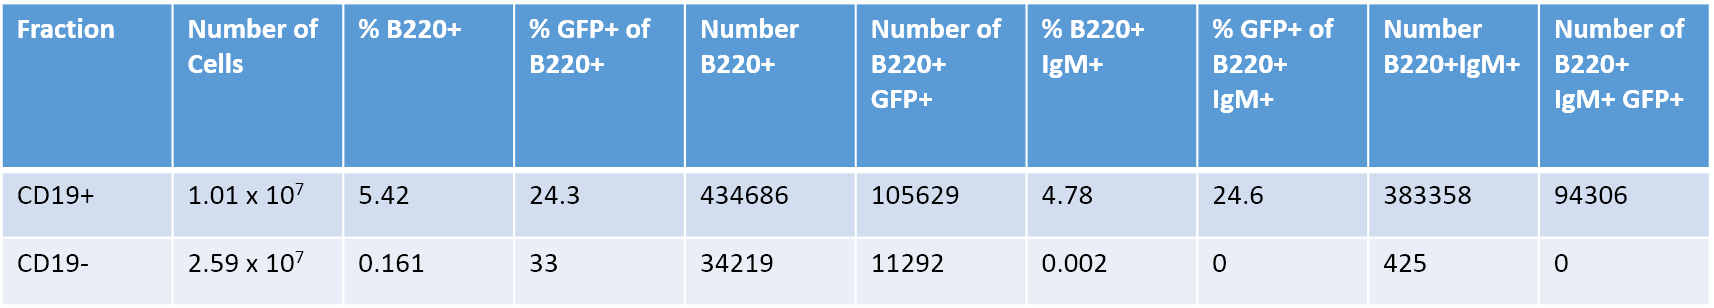
\includegraphics[width=\textwidth]{Figures/GFPdonortable.png}
	\end{subfigure}
\end{figure}

\begin{figure}
	\begin{subfigure}{0.45\textwidth}
	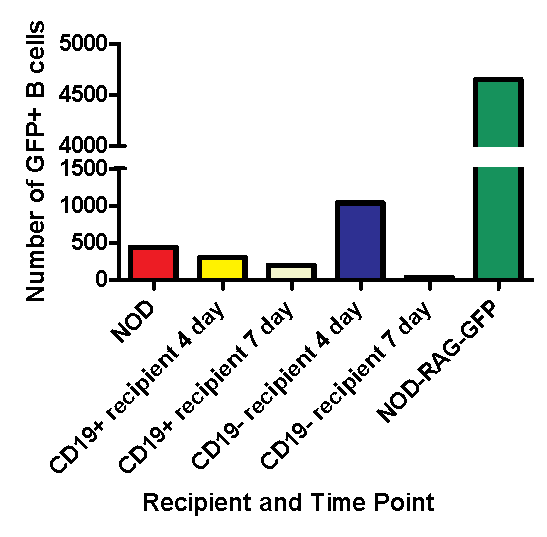
\includegraphics[width=\textwidth]{Figures/ThyGFPBcells.pdf}
	\caption{Thymus}
	\label{subfig:ThyGFPBcells}
	\end{subfigure}
	\begin{subfigure}{0.45\textwidth}
	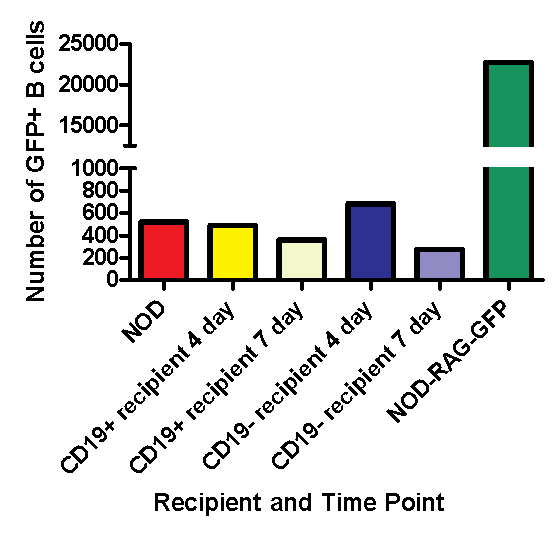
\includegraphics[width=\textwidth]{Figures/BMGFPBcells.pdf}
	\caption{Bone marrow}
	\label{subfig:BMGFPBcells}
	\end{subfigure}
	\begin{subfigure}{0.45\textwidth}
	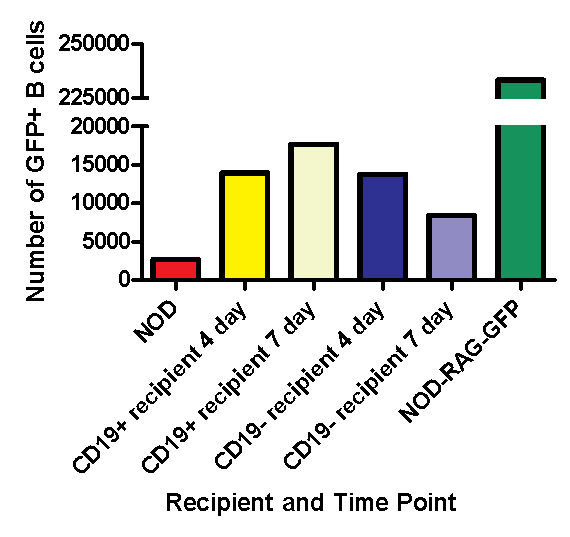
\includegraphics[width=\textwidth]{Figures/SpleenGFPBcells.pdf}
	\caption{Spleen}
	\label{subfig:SpleenGFPBcells}
	\end{subfigure}
	\begin{subfigure}{0.45\textwidth}
	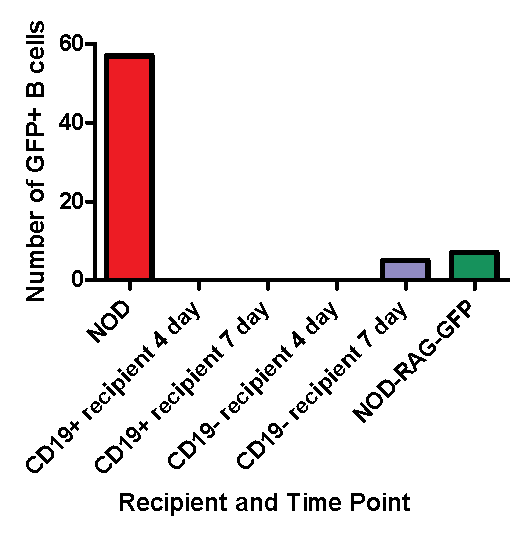
\includegraphics[width=\textwidth]{Figures/PLNGFPBcells.pdf}
	\caption{Pancreatic lymph node}
	\label{subfig:PLNGFPBcells}
	\end{subfigure}
	\begin{subfigure}{\textwidth}
	\centering
	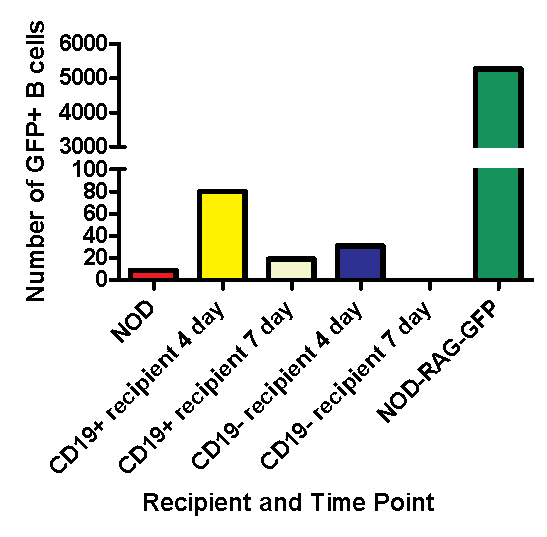
\includegraphics[width=0.45\textwidth]{Figures/axLNGFPBcells.pdf}
	\caption{Axillary lymph node}
	\label{subfig:axLNGFPBcells}
	\end{subfigure}
\caption{Graphs showing where transferred B cells migrate to.
Each graph shows the number of GFP\textsuperscript{+} B cells (CD19\textsuperscript{+}IgM\textsuperscript{+}) present in each tissue in each receipient/control. NOD WT control was included as a negative control as it has no GFP therefore any GFP\textsuperscript{+} B cells can be classed as `noise'. 
NOD-RAG-GFP was included as a positive control. 
Recipient mice were analysed at 4 and 7 days post transfer. n=1 for each group.}
\label{fig:GFPBcellgraphs}
\end{figure}

The results obtained from this experiment suggests that transferred B cells will only migrate to the thymus, spleen and axillary lymph node, as shown in \cref{fig:GFPBcellgraphs}.

Firstly, in the thymus, no GFP\textsuperscript{+} B cells were seen in the CD19\textsuperscript{+} recipient at either time point, shown by the numbers being less than that seen in the NOD WT control, see \cref{subfig:ThyGFPBcells}.
However, the total number of cells in the thymus of each mouse was also different (NOD WT 8.8 x 10\textsuperscript{6}, 4 day CD19+ recipient 4.8 x 10\textsuperscript{6}, 4d CD19- recipient 9.8 x 10\textsuperscript{6}, 7d CD19+ recipient 3.1 x 10\textsuperscript{6}, 7d CD19+ recipient 5.1 x 10\textsuperscript{6}, NOD-RAG-GFP control 7.3 x 10\textsuperscript{6}).
This shows that there are about double the number of thymic cells in the NOD compared to the CD19\textsuperscript{+} recipients at either time point, suggesting that the lower number of GFP+ B cells could be accounted for by the smaller number overall.
This decrease in total thymus cell number may be due to the mouse itself or the preparation of the thymus.
The other recipients have more similar total thymus cell numbers and are therefore more comparable.
Only the CD19\textsuperscript{-} recipient shows an increase in GFP\textsuperscript{+} B cells and even then, only at the 4 day time point.

In the bone marrow, \cref{subfig:BMGFPBcells}, all the recepients look very similar to the NOD control mouse, suggesting that any GFP\textsuperscript{+} B cells seen there are maybe just attributable to noise.

The spleen, showever, does show an increase in GFP\textsuperscript{+} B cells in all recipients at all time points compared to NOD control, \cref{subfig:SpleenGFPBcells}. 
This is interesting as it suggests that transferred GFP\textsuperscript{+} B cells are migrating to the spleen to develop, as would conventional B cells.
The total thymus cell count for the NOD WT is about the same as the 7 day CD19\textsuperscript{-} recipient (~3.7 x 10\textsuperscript{6} cells), which is about half the number of cells in each of the other mice.
However, the number of GFP\textsuperscript{+} B cells seen in all recipient mice is increased compared to the NOD mouse suggesting that the difference cannot be accounted for by the difference in thymus cell number.

In the pancreatic lymph node, \cref{subfig:PLNGFPBcells}, it appears that there is a lot of `noise' in the NOD control as this mouse should not have any GFP and yet the number of GFP\textsuperscript{+} B cells is supposedly far greater than that seen in the NOD-RAG-GFP positive control. 
It seems that there are no GFP\textsuperscript{+} B cells in any recipients, and that this is reasonable due to the very small number seen in the NOD-RAG-GFP positive control mouse.

Finally, in the axillary lymph node \cref{subfig:axLNGFPBcells}, it appears that GFP\textsuperscript{+} B cells are only seen in the CD19\textsuperscript{+} and potentially CD19\textsuperscript{-} recipients at the 4 day time point.
The total cell counts for each recipient and control were all fairly similar therefore it appears that any differences in GFP\textsuperscript{+} B cells cannot be accounted for by differences there.

Overall it appears that GFP\textsuperscript{+} B cells migrate mainly to the spleen, with a some migrating to the thymus and axillary lymph node.
This suggests that thymic derived B cells do not on the whole migrate back to the thymus following transfer.
However, in the thymus, the CD19\textsuperscript{-} recipient is the only one to show an increase in GFP\textsuperscript{+} B cells. 
This could be due to chance or contaminating B cells, or it may be due to the fact that this fraction contains CD19\textsuperscript{-} B cell progenitors which may need to be in the thymus to develop into B cells.
This could indicate that thymic B cells need to develop initially in the thymus, but following this, they can continue development in the spleen, similar to conventional B cells.
In order to investigate this further, the group size would need to be significantly increased to see whether this difference is due to chance or is a real observation.



\subsection{Autoantibody production}

The purpose of this experiment was to look for any autoantibodies present in the serum of a NOD mouse.
To do this, thymi were first depleted of all CD45\textsuperscript{+} cells to leave only stromal cells which were then transferred onto microscope slides and incubated either in NOD WT serum or PBS.
Subsequent staining with anti-mouse antibody revealed any antibodies bound to thymic stroma.

Interestingly, as shown in \cref{subfig:WTserum}, there appeared to be intracellular staining seen only on the serum treated sample.
The PBS incubated sample showed no such staining, \cref{subfig:WTcontrol}.

This pattern of staining suggests that the NOD WT mouse may produce an antibody specific to an intracellular component of thymic stromal cells.
However, it is not possible to say what the antibody is specfic for and further investigation would be needed to determine this.
However, mTECS and cTECS present in the thymus are important mediators of positive and negative selection, therefore if antibodies are present to any components relating to these processes, it may be that they are affecting the efficient education of T cells.

This experiment was carried out as a very preliminary experiment to see if it was worth further investigation and the results suggest that it is.
Possible things to try include:
\begin{itemize}
\item Increasing group size from one thymus
\item Try incubating NOD WT stroma in B6 serum to see if the antibody binding is specific to the NOD serum
\item Try incubating B6 serum with NOD serum to see if the antigen is specific to the NOD mouse
\end{itemize}

If the action of the autoantibodies is thought to implicate the process of negative selection, it may be of use to use mice that have various components relating to this process knocked out.
For example, an AIRE knock out mouse could potentially show whether the autoantibodies are specific to an AIRE-related component.


\begin{figure}
	\begin{subfigure}{\textwidth}
		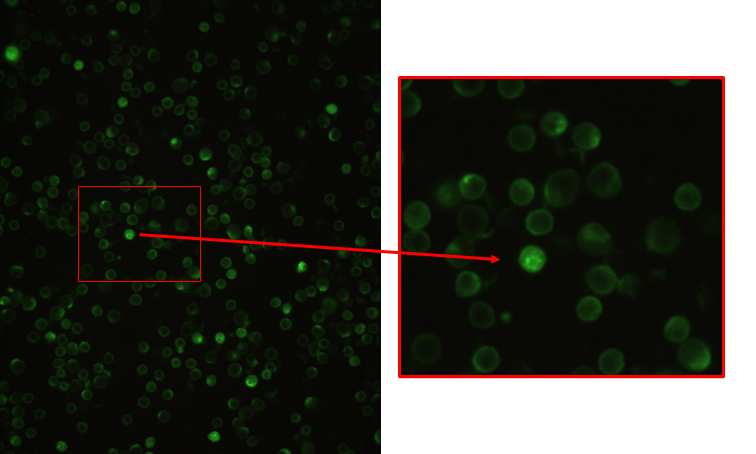
\includegraphics[width=\textwidth]{Figures/WTserum.png}
		\caption{Serum treated}
		\label{subfig:WTserum}
	\end{subfigure}
	\begin{subfigure}{\textwidth}
		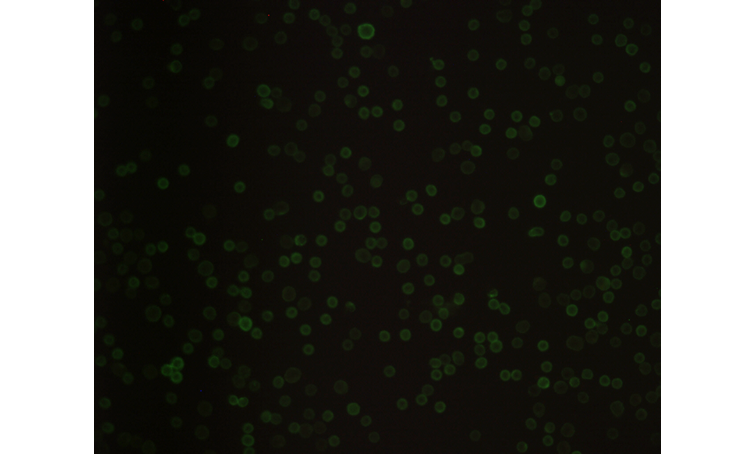
\includegraphics[width=\textwidth]{Figures/WTcontrol.png}
		\caption{PBS treated}
		\label{subfig:WTcontrol}
	\end{subfigure}
\caption{This image shows NOD WT thymic stroma incubated with serum from a 16 week old NOD WT mouse (top) and NOD WT stroma incubated with PBS as a control (bottom).
Following incubation with serum or PBS, samples were stained with anti-mouse antibody conjugated to FITC.
Slides were imaged using...}
\label{fig:histology}
\end{figure}


\subsection{Conclusion}

Following the data obtained above, it appears that B cells derived from the thymus don't have a strong preference for migrating back to the thymus following transfer and instead, most migrate to the spleen.
This could suggest that the function of a thymic B cell is in the spleen, or that thymic B cells do not have the ability to return to the thymus either once they have been removed from the thymus, or following transfer (for example, the necessary features required to home to the thymus may be lost during transfer).

In terms of histology, it appears that there are autoantigens present in the NOD thymus that are specific for an intracellular component of thymic stromal cells.
However, it is not possible to tell what the antigen is.
It is necessary to repeat this experiment to increase the group size and consider other strains of mice and other controls.
This would then increased the validity of the results obtained and decrease the posisbility that the findings are as a result of chance.
